	% !TEX encoding = UTF-8 Unicode

	\documentclass[a4paper]{article}

	\usepackage{color}
	\usepackage{url}
	\usepackage[T2A]{fontenc} % enable Cyrillic fonts
	\usepackage[utf8]{inputenc} % make weird characters work
	\usepackage{graphicx}
	\usepackage{amsmath}
	\usepackage{amssymb}


	\usepackage[english,serbian]{babel}
	%\usepackage[english,serbianc]{babel} %ukljuciti babel sa ovim opcijama, umesto gornjim, ukoliko se koristi cirilica

\usepackage[ruled,vlined]{algorithm2e}

\newenvironment{megaalgorithm}[1][htb]
  {\renewcommand{\algorithmcfname}{Algoritam}% Update algorithm name
   \begin{algorithm}[#1]%
  }{\end{algorithm}}


	\usepackage[unicode]{hyperref}
	\hypersetup{colorlinks,citecolor=green,filecolor=green,linkcolor=blue,urlcolor=blue}

	%\newtheorem{primer}{Пример}[section] %ćirilični primer
	\newtheorem{primer}{Primer}[section]
	\newtheorem{definicija}{Definicija}[section]

	\begin{document}

	\title{Uvod u temporalne logike i njihova primena u proveravanju modela\\ \small{Seminarski rad u okviru kursa\\Metodologija stručnog i naučnog rada\\ Matematički fakultet}}

	\author {Đorđe Todorović  mi12090@alas.matf.bg.ac.rs, \\ Stefan Zarić mi12147@alas.matf.bg.ac.rs, \\ Maksim Đurđevac  mi11362@alas.matf.bg.ac.rs}
	\date{8.~april 2017.}
	\maketitle

	\abstract{
	Seminarski rad obrađuje temu \emph{Temporalne logike}, tačnije upotrebu logike u računarstvu za čiju upotrebu
	veoma bitnu ulogu ima vreme.
	Preciznije su opisane osnove \emph{Linearne temporalne logike (LTL)} i \emph{Logike stabla 
	izračunavanja (CTL)}, osnovne primene ovih logika, a takođe su navedeni i najpoznatiji alati za proveravanje modela,
	kao i mogućnosti alata ESBMC.
	\tableofcontents

	\newpage

	\section{Uvod}
	\label{sec:uvod}

	Glavni cilj upotrebe logike u računarstvu je da se razviju jezici koji modeluju situacije koje srećemo kao profesionalci u toj oblasti, ali u nekom formalnom obliku. Glavni cilj je zadati formalna pravila za ispitivanje validnosti zadatih argumenata.
	 
	Uska je povezanost pojmova \emph{Temporalna logika} i \emph{Iskazna logika}, gde takođe imamo jasno definisanu sintaksu i semantiku. Jezici u matematici su pretežno simbolički, sto će reći da kombinovanjem istih dobijamo izraze koji predstavljaju određene matematičke objekte. Sintaksa jezika definiše skup validnih simbola koji se mogu upotrebljavati i kombinovati kako bi se kreirali takođe validni izrazi. Semantika se bavi tumačenjem izraza. Iskazna logika (i predikatska logika) je dobra za opisivanje matematičkih problema koje srećemo u teoriji, ali često imamo potrebu za opisivanjem i modelovanjem problema koje srećemo svakodnevno u životu.
	
	Temporalne logike su logike koje opisuju rezonovanja u kojima je uklju-čeno i vreme. Primena ovih logika je sve veća kako kod softverskih rešenja, tako i kod kreiranja samog hardvera. One su sve značajnije u oblasti Informacionih tehnologija, tj. računarstvu, jer se ponašanje i hardvera i softvera opisuje u zavisnosti od vremena. Preko njih se između ostalog opisuje i rad operativnih sistema, funkcionisanje konkurentnih sistema, rad procesora, memorije itd. Vreme u Temporalnoj logici modelujemo upotrebom različitih operatora. Osnovne vrste ovih logika jesu \emph{Linearne temporalne logike (LTL)} i \emph{Logike stabla odlučivanja (CTL)}, a u daljem tekstu će ove dve vrste biti detaljnije obrađene.

	\section{Linearne temporalne logike}
	\label{sec:LTL}

	%\newline
	Kao što smo već napomenuli, Temporalne logike uključuju u razmatranje vreme, a takođe smo pomenuli i neke osnovne vrste ovih logika, pa stoga ćemo prvo opisati LTL model, Linearne temporalne logike, koje vreme posmatraju kao sekvence koje se linearno ređaju jedna za drugom. Linearne temporalne logike predstavljaju beskonačan niz sekvenci gde u svakom trenutku svaka od njih ima svog naslednika, na osnovu linearne vremenske perspektive. Uvodimo i pojam \emph{linearno temporalno svojstvo} (\emph{LT svojstvo}) koje predstavlja temporalnu logičku formulu koja opisuje skup beskonačnih sekvenci koje su tačne, tj. imaju vrednost \emph{True} \cite{reeves1990logic}.

	Svrha LTL-a jeste da se svojstva napisana u prirodnom jeziku prevedu u LTL uz pomoć precizno definisane sintakse. Ovu logiku odlikuje pojava različitih operatora, čijom upotrebom možemo opisati razne modele vremena, ali nama će za sada biti interesantni samo operatori koji opisuju linearne sekvence. Postoje i tzv. univerzalni logički veznici, kojima možemo opisati svaku vrstu  Temporalnih logika \cite{reeves1990logic}.
	\subsection{Sintaksa}
	\label{subsec:podnaslovN}
%	\newline
	
Sintaksa proučava pravila koja određuju kako se strukturni elementi jezika na pravilan način mogu kombinovati i stvarati takođe ispravan složeniji element. Kombinacijom operatora i atoma dobijamo logičke formule.%\newline

Formula Linearne temporalne logike je sačinjena od: 
\begin{enumerate}
\item  Konačnog skupa atoma $(a, b, x, y, ....)$
\item  Osnovnih logičkih operatora ($\neg$ (negacija (eng. \emph{negation})) , $\wedge$ (konjukcija (eng. \emph{conjunction}))) 
\item  Osnovnih temporalnih operatora (O (next) , U (until) , true) 
\item  Postoje i dodatni logički operatori ($\vee$ (disjunkcija (eng. \emph{disjunction})), $\rightarrow$(implikacija (eng. \emph{implication})), $\leftrightarrow$(ekvivalencija (eng. \emph{equivalence})))
\item  Postoje i dodatni temporalni operatori ( A (”always”), E (”eventually”))
\end{enumerate}

	Kombinacijom navedenih možemo dobiti složenije operatore. Stoga ćemo navesti još neka pravila:
\begin{enumerate}	
\item $\square \rightarrow 'F'$, što znači nešto konačno u budućnosti 
\item $\lozenge \rightarrow 'G'$, što znači nešto globalno u budućnosti 
\item $\circ \rightarrow 'X'$, što znači nešto sledeći put 
\end{enumerate}

	LTL može biti prošireno sa operatorima prošlosti: 
\begin{enumerate}	
\item $\square^{-1} \rightarrow $ Uvek u prošlosti 
\item $\lozenge^{-1} \rightarrow $  Ponekad u prošlosti 
\item $\circ^{-1} \rightarrow $ Prethodna sekvenca 
\end{enumerate}

   Takođe ćemo napomenuti i pravila 'weak until' i 'release':
\begin{enumerate}	
\item  Weak until (a W b)

		-a ostaje True dok b ne postane True, pri tom može zauvek ostati True (ne zahteva se da b ikad postane True)
\item   Release (a R b) 

		-b ostaje True dok a ne postane True, pri tom može zauvek ostati True (ne zahteva se da b ikad postane True) znači suprotno od prethodnog.
\end{enumerate}		

	\subsection{Semantika}
	\label{subsec:podnaslovN}
	
	Sintaksa logike definiše kako nešto možemo zapisati ispravno, a semantika daje značenje istom.
	Vrste sistema koje obično modelujemo uz pomoć LTL-a nazivamo \emph{Tranzicionim sistemima (TS)}. Razaznajemo pojmove \emph{stanje} (eng. \emph{state}), što predstavlja statičku strukturu i \emph{tranzicija}(eng. \emph{transition}) , što predstavlja dinamičku strukturu. TS predstavlja skup stanja S povezanih tranzicionom relacijom $\rightarrow $(binarna relacija na S) \cite{reeves1990logic}.
	
	LTL formula $\varphi$ označava svojstva stanja, dok jedno konkretno stanje može biti potpuna LTL formula, a i ne mora.
	
	Semantika formule $\varphi$ je definisana kao jezik($\varphi$) gde on sadrži beskonačnan skup reči koje zadovoljavaju $\varphi$.
	
	Radi lakšeg razumevanja značenja Temporalnih logika navešćemo neke opšte definicije logike, koje između ostalog važe i za Linearne temporalne logike.

	Kao i u klasičnoj iskaznoj logici, ako je A neka formula, onda zapis $A = A(p_1, p_2, \dots , p_n)$ znači da su sva iskazna slova formule $A$ u skupu $\{p_1, p_2, \dots , p_n\}$.
\begin{definicija}
Neka je $A = A(p_1, p_2, \dots , p_n)$ neka LTL formula. Interpretacija te formule je svaki uređen par $I = (S, \rho)$, gde je $S$ skup svih valuacija $s : \{p_1, p_2, \dots , p_n\} \to \{>, \perp \}$, tzv. stanja, a $\rho \subset S2$ binarna relacija na skupu stanja (tzv. funkcija prelaska).
\end{definicija}
\begin{definicija}    
Neka je $A = A(p_1, p_2, \dots , p_n)$ neka LTL formula, $I = (S, \rho)$ neka interpretacija formule $A$, i $s \in S$. Tada definišemo $v_I$, $s(A) \in \{>, \perp \}$, tzv. vrednost formule $A$ za interpretaciju $I$, u stanju $s$, na sledeći način:
\begin{enumerate}	
\item  Ako je $p \in P$ onda $v_I,s(p) = s(p)$
\item $v_I,s(\not B) = \top$ akko $v_I,s(B) = \bot$
\item  $v_I,s(B \vee C) = v_I,s(B) \wedge v_I,s(C)$
\item  $v_I,s(B \vee C) = v_I,s(B) \wedge v_I,s(C)$
\item $v_I,s(B \Rightarrow C) = v_I,s(B) \Rightarrow v_I,s(C)$
\item $v_I,s(B \Leftrightarrow C) = (v_I,s(B) \Leftrightarrow v_I,s(C))$
\item  $v_I,s(\square B) = \top$ akko $v_I,t(B) = \top$, za sve $t \in (s)$
\item $v_I,s(\diamond B) = \top$ akko $v_I,t(B) = \top$, za neki $t \in \rho(s)$.
\end{enumerate}	
Ukoliko je $v_I,s(A) = \top$, pišemo $I, s \models A$ ili samo $s \models A$. U suprotnom pišemo $I, s \nvDash A$.
\end{definicija} 
\begin{definicija}
Neka je A neka LTL formula. Tada:
\begin{enumerate}	
\item Kažemo da je A zadovoljiva ako postoji interpretacija $I = (S, \rho)$ za A i neko stanje $s \in S$ tako da je $v_I,s(A) = \top$ tj. $I, s \models A$.
\item Ako je $I = (S, \rho)$ i postoji $s \in S$ tako da je $I, s \models A$, onda kažemo da je I model za A i pišemo $I \models A$.
\item Formula A je LTL-valjana ako za sve interpretacije $I = (S, \rho)$ i sva stanja $s \in S$, važi $I, s \models A$. U tom slučaju pišemo $\models A$.\end{enumerate}	
\end{definicija}

	TS zadovoljava LT svojstvo P ako sva njegova stanja zadovoljavaju P, tj. ako sva njegova ponašanja jesu prihvatljiva. A stanje zadovoljava P kad god sva stanja koja su proizišla iz njega zadovoljavaju P. TS zadovoljava  $\phi$ ako TS zadovoljava LT svojstva definisana na Jezik($\phi$) \cite{reeves1990logic}.


	\section{Logike stabla izračunavanja}
	\label{sec:CTL}
	U LTL analizi smo zapazili da je LTL formula evaluirana preko stanja. Definisali smo da stanje sistema
	zadovoljava jednu LTL formulu ako sva stanja koja proizilaze iz njega zadovoljavaju istu. CTL(eng. \emph{Computation tree logic}) je logika koja je predstavljena strukturom drveta i u njoj budući koraci još nisu
	određeni, jer postoji više stanja koja potencijalno mogu biti "iskorišćena".
	CTL nam omogućava da prebrodimo neke nedostatke LTL metoda. Kao i u LTL, imamo operatore U, F, G i X, takođe imamo i kvantifikatore
	A i E koji opisuju sva stanja(eng. \emph{all states}) i postojeća stanja (eng. \emph{exists states}). 

\subsection{Sintaksa}
	\label{subsec:podnaslovN}
	CTL koristi logiku stabla pri izračunavanju. 
	Kao pre, radimo sa konačnim skupom atomičkih formula (kao što su $p, q, r,...,p_1,p_2,p_3...$).

	Definišemo CTL formulu:
\begin{equation}
\begin{split}
\phi := &\top| \bot | p | (\neg \phi) | (\phi \wedge \phi) | (\phi \vee \phi) | (\phi \rightarrow \phi)| AX\phi | EX\phi | \\
          &  AF\phi | EF\phi | AG\phi | EG\phi | A[\phi \cup \phi] | E[\phi \cup \phi]
\end{split}
\end{equation}
	gde je $p$ iz konačkog skupa atomičkih formula.
	%\newline
	
	\subsection{Semantika}
	\label{subsec:podnaslovN}
	CTL formula je interpretirana preko tranzicionog sistema (TS). Neka je $M = (S,\rightarrow, L)$ neki model, $s \in S$ i $\phi$ CTL formula.
	Definicija modela bi bila sledeća:
	\begin{enumerate}	
\item Ako je $\phi$ atomička, zadovoljivost je razrešena preko L.
\item  Ako veznik najvišeg prioriteta formule $\phi$ je bulovski veznik tada se pitanje zadovoljivosti razrešava
		   preko uobičajne istinitosne tablice i rekurzije nad drvetom formule $\phi$.
\item  Ako je veznik najvišeg prioriteta neki operator koji počinje sa A, tada zadovoljivost jeste ispunjena ako
		   sva stanja iz s zadovoljavaju LTL formulu koja se dobija kada izbacimo simbol A.
\item  Slično ako je veznik najvišeg prioriteta neki operator koji počinje sa E, tada zadovoljivost jeste ispunjena ako
		   sva stanja iz s zadovoljavaju LTL formulu koja se dobija kada izbacimo simbol E.
\end{enumerate}	

	\section{Primena temporalnih logika u proveravanju modela}
	\label{sec:MC}
	Sada kada smo se upoznali sa osnovama LTL-a i CTL-a, prikazaćemo njihove primene u proveravanju modela.
\subsection{LTL}
	\label{subsec:prLTL}
	Linearna temporalna logika ima primenu u formalnoj verifikaciji sistema, pre svega u konkurentnim programima gde je bitno utvrditi da se program ne može naći u stanju mrtve petlje \cite{baier2008principles}. 
	
	Provera modela je tehnika za automatsku verifikaciju softvera i hardvera. Proverava se da li sistem ispunjava specifikaciju koja je zadata formulom linearne temporalne logike. 
	Svaki zahtev u specifikaciji može se predstaviti jednom formulom linearne temporalne logike i može se nezavisno proveriti da li je ispunjen za dati sistem. Konjunkcija svih zahteva predstavlja specifikaciju sistema.
	Program predstavljamo kao konačni automat, i proveravamo da li je formula temporalne logike tačna u toj strukturi, odnosno da li program ispunjava specifikaciju.
	Algoritam linearne temporalne logike za proveru modela je procedura koja vraća ,,da'' za dati tranzicioni sistem $TS$ i formulu $\phi$ ako je $TS \vDash \phi$, odnosno ,,ne'' ako $TS$ nije model formule $\phi$.

	Prednosti i mane korišćenja provere modela.

	Prednosti: 
\begin{itemize}
\item Nema potrebe za formalnim dokazima korektnosti. 
\item  Brzina, u poređenju sa drugim metodima verifikacije. 
\item Ako specifikacija nije zadovoljena biće generisan kontraprimer koji će pokazati kako se došlo u to stanje i onda se može zaključiti zašto specifikacija nije ispunjena. 
\item Moguće je proveriti ispunjenost zahteva i pre nego što je ceo sistem završen, tako da se može vršiti provera modela tokom izrade većeg sistema. 
\item Korišćenjem linearnih temporalnih logika mogu se iskazati svojstva konkurentnih programa koja su nam potrebna u automatskoj verifikaciji. 
\end{itemize}	
	Mane: 
\begin{itemize}	
\item Zadavanje specifikacija formulama linearne temporalne logike može da bude komplikovano. 
\item Pisanje specifikacija je teško i mali broj inženjera je obučen za formalnu verifikaciju sistema. 
\item  Broj stanja u kome sistem može da se nađe može biti izuzetno velik, pogotovu ako radimo proveru modela na sistemima na kojima imamo konkurentnost. 
\end{itemize}	


Algoritam za proveru modela upotrebom automata i linearne temporalne logike je naveden u algoritmu \ref{alg:katl}. O nedeterminističkim Buhijevim automatima (NBA) koji se koriste u ovom algoritmu može se pročitati u \cite{alur1994theory}.

\begin{megaalgorithm}
\caption{Algoritam za proveru modela upotrebom automata i linearne temporalne logike}\label{alg:katl}

\textbf{Ulaz: }konačni automat (tranzicioni sistem $TS$) i LTL formula $\phi$ 

\textbf{Izlaz:} DA ako je $TS \vDash \phi$; inače, NE i generisan kontraprimer 

\Indp Konstruisati NBA $A\neg\phi$ tako da $L_\omega (A\neg \phi) = Words(\neg \phi)$

	Konstruisati tranzicioni sistem $TS\circ A$ 

	\textbf{if} postoji put $n$ u $TS \circ A$ koji zadovoljava uslov ispunjenosti $A$ \textbf{then} 

		\Indp \textbf{return} NE i odgovarajući prefiks od $n$ 
	
	\Indm \textbf{else} 

		\Indp \textbf{return} DA 
		
	\Indm \textbf{fi}
\end{megaalgorithm}

U praksi se koriste alati za proveravanje modela koji implementiraju neki od algoritama za proveravanje modela. Ovi programi obično rade tako što zahteve zadate LTL formulama pretvaraju u konačne automate. Kao što se vidi u algoritmu \ref{alg:katl} uzima se negacija LTL formule i pravi se automat nad njom, zatim se napravi proizvod dobijenog automata i automata koji predstavlja sistem i vrši se provera ispunjenosti uslova \cite{gastin2001fast}.

Jedan primer kako se LTL formulom može zadati zahtev je sledeći. Ako posmatramo problem dodele nedeljivih resursa procesima u operativnom sistemu, i formula $\alpha$ predstavlja zahtev za resursom a formula $\beta$ predstavlja realizaciju tog zahteva, onda formula $G(\alpha \rightarrow F \beta)$ označava da će svaki zahtev za resursom biti opslužen \cite{formverif}.

Još jedan primer je raspoređivanje procesa. Ako formula $\alpha$ predstavlja početak rada procesa A, a formula $\beta$ kraj rada procesa B, onda formula $(\neg\alpha)\cup\beta$ znači da završetak rada procesa B mora prethoditi početku rada procesa A \cite{formverif}.

% Spin je jedan od  alata za verifikaciju softvera koji podržava zadavanje zahteva LTL formulama\cite{holzmann1997model}. Zanimljiv primer gde je korišćen Spin je raspoređivanja procesa na distribuiranom operativnom sistemu. Na slici \ref{fig:dsps} je dat tranzicioni sistem koji je Spin generisao.

%\begin{figure}[h!]
%\begin{center}
%\includegraphics[scale=1.0]{dsps.png}
%\end{center}
%\caption{Tranzicioni sistem za klijent (levo) i server (desno)}
%\label{fig:dsps}
%\end{figure}

\subsection{CTL}
	\label{subsec:prCTL}
	
Kao što je već ranije pomenuto izražajnost LTL i CTL nije jednaka \ref{fig:ltlctlex}. Iz tog razloga i CTL su našle svoju primenu u proveravanju modela \cite{rozier2011linear}. Dakle model sistema je dat kao struktura, konačan automat, a specifikacija zahteva sistema je zadata formulama CTL-a.  Glavna tehnika koja se ovde koristi za proveru modela je obilazak grafa pretagom u širinu \cite{abate2007one}.

\begin{figure}[h!]
\begin{center}
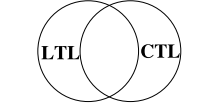
\includegraphics[scale=1.5]{ltlctl.png}
\end{center}
\caption{Izražajnost LTL i CTL}
\label{fig:ltlctlex}
\end{figure}

Algoritam \ref{alg:kaCTL} predstavlja algoritam za proveru modela upotrebom automata i logike stabla izračunavanja i prvi put je u tom obliku prikazan u radu \cite{rozier2011linear} .

\begin{megaalgorithm}
\caption{Algoritam za proveru modela upotrebom automata i logike stabla izračunavanja}\label{alg:kaCTL}
\textbf{Ulaz: }konačni automat (tranzicioni sistem $TS$) i CTL formula $\phi$ 

\textbf{Izlaz:} DA ako je $TS \vDash \phi$; inače, NE i generisan kontraprimer 

\Indp  Definisati model sistema $M$ koji sadrži putanje do svih stanja na osnovu skupa svih zahteva $Prop$

	Neka je $\phi$ CTL formula kojom su zadati zahtevi iz skupa $Prop$ 

	Proveriti da $M \vDash \phi$

		\Indp Prevesti specifikaciju $\neg\phi$ u Buhijev automat  $A_{\neg\phi}$ i spojiti ga sa modelom sistema $M$ da bi se formirao sistem $A_{M, \neg\phi}$
		
		Proveriti da li je $A_{M, \neg\phi}$ neprazan pretragom putanja koje prihvata $A_{M, \neg\phi}$
		
		\textbf{if}  putanja koje prihvata $A_{M, \neg\phi}$ postoji
		
		\Indp \textbf{return } NE i putanju kao kontraprimer
		
		\Indm  \textbf{else}	

		\Indp \textbf{return } DA

	\Indm \textbf{fi}
\end{megaalgorithm}

	\section{ESBMC verifikacioni alat}
	\label{sec:ESBMC}
Verifikacija softvera može imati različite primene.  Najčešća primena alata za verifikaciju je u oblasti  gde je ispravnost programa izrazito važna. U nastavku su prikazani neki od najpoznatijih alata (Tabela 1).


\begin{table}
\begin{center}
 \begin{tabular}{||c c ||} 
 \hline
 \textbf{Alat}  & \textbf{Platforma / Operativni sistem} \\ [0.5ex] 
 \hline\hline
 \href{https://altarica.labri.fr/wp/} {ARC} & Unix \\ 
 \hline
 \href{http://bandera.projects.cs.ksu.edu/} {BANDERA} & Windows i Unix  \\
 \hline
 \href{https://en.wikipedia.org/wiki/BLAST_model_checker/} {BLAST}  & Windows i Unix  \\
 \hline
 \href{http://www.kenmcmil.com/smv.html} {CADENCE SMV} & Windows i Uni  \\
 \hline
 \href{https://en.wikipedia.org/wiki/Construction_and_Analysis_of_Distributed_Processes} {CADP} & Mac OS, Linux, Solaris, Windows  \\
  \hline
 \href{http://www.cprover.org/cbmc/} {CBMC} & Windows i Unix \\ 
  \hline
 \href{https://cpachecker.sosy-lab.org/} {CPAchecker} & Svi \\ 
  \hline
 \href{http://www3.cs.stonybrook.edu/~cwb/} {CWB-NC} & Windows,Unix, Mac OS \\ 
  \hline
 \href{http://divine.fi.muni.cz/} {DIVINE} & Unix \\ 
  \hline
 \href{https://en.wikipedia.org/wiki/DREAM_(software)} {DREAM} & Windows i Unix \\ 
  \hline
 \href{http://dsverifier.org/} {DSVerifier} & Windows i Unix \\ 
   \hline
 \href{http://www.cprover.org/ebmc/} {EBMC} & Windows i Unix \\ 
   \hline
 \href{http://homepages.inf.ed.ac.uk/perdita/cwb/} {Edinburgh CWB} & Windows i Unix \\ 
   \hline
 \href{https://www.btc-es.de/en/} {EmbeddedValidator} & Window \\ 
   \hline
 \href{https://fldit-www.cs.uni-dortmund.de/~peter/ExpNeu/Welcome.html} {Expander2} & Unix \\ 
   \hline
 \href{http://www-sop.inria.fr/meije/verification/} {Fc2Tools} &  Unix \\ 
   \hline
 \href{http://jabc.cs.tu-dortmund.de/modelchecking/} {GEAR} & Windows i Unix \\ 
   \hline
 \href{https://github.com/tomahawkins/improve/wiki/ImProve} {ImProve} & Windows i Unix \\ 
   \hline
 \href{https://en.wikipedia.org/wiki/Java_Pathfinder} {Java Pathfinder} &  Windows,Unix, Mac OS \\ 
   \hline
 \href{http://llbmc.org/} {LLBMC} & Windows i Unix \\ 
    \hline
 \href{http://www.doc.ic.ac.uk/~jnm/book/} {LTSA} & Windows i Unix \\ 
     \hline
 \href{http://fmt.cs.utwente.nl/tools/ltsmin/} {LTSmin} & Unix, Mac OS , Windows \\
    \hline
 \href{https://en.wikipedia.org/wiki/PRISM_model_checker} {PRISM} &  Windows,Unix, Mac OS \\
   \hline
 \href{http://www.cprover.org/satabs/} {SATABS} &  Windows i Unix \\ [1ex]
 \hline
\end{tabular}
\caption{Verifikacioni alati \cite{wikiwebsite}}
\end {center}
\end {table}


\newpage


	U dizajnu kompleksnih softverskih sistema više se truda i vremena potroši na
	verifikaciju nego na konstrukciju samog softvera. Verifikacione tehnike  zasnovane na modelima se baziraju na modelima koji opisuju ponašanje sistema na matematički precizan i nedvosmislen način. Ispostavilo se da pre bilo kakvih verifikacionih provera, precizno modelovanje sistema često dovodi do otkrivanja nepravilnosti, nepotpunosti i nelogičnosti u neformalnim specifikacijama sistema. Takvi problemi se obično otkrivaju u kasnim fazama dizajna. Modeli sistema su praćeni algoritmima koji sistematično istražuju sva njihova stanja. To je preduslov za čitav niz tehnika verifikacije polazeći od provera modela preko simulacije do testiranja.
	Provera modela je verifikaciona tehnika koja istražuje sva moguća stanja sistema koristeći brute-force način.
	\newline

\textbf{ESBMC} je kontekstno-ograničeni kontrolor modela ugrađen u $C$ i $C++$ softver, baziran na SMT (eng. \emph{satisfiability modulo theory}) rešavaču.  On dozvoljava verifikacionom inženjeru da: 
	\newline
	\begin{enumerate}
	\item Verifikuje jednonitni i višenitni softver (sa deljenim promenljivama i međusobnim isključenjem);
	\item Prosuđuje o aritmetičkim prekoračenjima, bezbednosti pokazivača, curenju memorije, granicama nizova, kršenju atomičnosti i redosleda izvršavanja, mrtvim blokadama i utrkivanjima; 
	\item Verifikuje programe koji koriste aritmetiku na nivou bita, pokazivača, struktura, unija i sa fiksnim zarezom.
	\end{enumerate} 
	ESBMC ne zahteva od korisnika da komentariše programe sa preduslovima i postuslovima (eng. \emph{pre/post-conditions}), već mu dozvoljava da navede dodatna svojstva koristeći assert-instrukcije, koje se potom kontrolišu. Takođe, obezbeđuje tri pristupa (lenji, snimanje po rasporedu, podaproksimaciju i proširivanje) za kontrolu modela višenitnog softvera. ESBMC može biti pozivan kroz tekstualni komandni interfejs ili podešen putem dodatka za Eclipse. ESBMC obrađuje verifikacione uslove koristeći različite pozadinske teorije i prosleđuje ih direktno u SMT rešavač. \cite{esbmc} 
	\newline
	Podrazumevano, ESBMC proverava da li ima nepravilnosti u samom programskom jeziku, po ISO/ANSI programskom standardu. Naravno, program može da bude ispravan, ali da ima pogrešnih stvari. Kod takvih slučajeva se dodaju dodatne specifikacije za program koristeći assert instrukcije. 
	\newline
	ESBMC  koristi transformacije  da pretvori program u niz matematičkih ograničenja:
	\begin{enumerate}
	\item Komponente biblioteka su objedinjene u programski tekst.
	\item Kontrola toka se pretvara u jednostavnu GOTO formu.
	\item GOTO program se prevodi u formu  u kojoj se zahteva da je promenljivoj dodeljena vrednost tačno jednom i svaka promenljiva je definisana, pre korišćenja. U ovoj fazi smo se pomerili sa predstavljanja C promenljive u promenljivu koja algebarsku nepoznatu povezuje sa svakim izvršenjem jednog zadatka.
	\item Uvodimo dodatna ograničenja između nepoznatih, koja jedino mogu biti zadovoljena ako program ima grešku.
	\item SMT(eng. \emph{satisfiability modulo theory}) rešavač se pokreće da istraži da li sva ograničenja mogu biti zadovoljena odjednom. Bilo koji uspeh je greška u programu.
	\item Ako SMT solver uspe (program ne prolazi) koristimo njegovo uspešno dodeljivanje promenljive nepoznatoj da zaključimo pogrešan tok programa.
	\end{enumerate}
	Za ovaj primer programa:
	\newline
	\begin{primer}

\begin{verbatim}

	#include  <stdlib.h>  	
	
	int main()
	{
		unsigned int size = nondet_int();
		char *hunk = malloc(size); 
		unsigned int pos = nondet_int(); 
		hunk[pos] = 0;
		return 0;
	}
\end{verbatim}
	\end{primer}
	Generiše se sledeći izveštaj:
	\newline
	Violated property: file test.c line 10 function main dereference failure: dynamic object upper bound !(\_\_ESBMC\_is\_dynamic[POINTER\_OBJECT(hunk + pos)] \&\& DYNAMIC\_SIZE(hunk + pos) <= POINTER\_OFFSET(hunk) + pos) VERIFICATION FAILED

\cite{esbmc001}

	\section{Zaključak}
	\label{sec:zakljucak}

Greške su sastavni deo svakog rada, te je njihovo pojavljivanje u računa-rstvu sasvim uobičajno. Glavni cilj je iste te greške detektovati i otkloniti na vreme, pre nego što postanu pretnja po čitav sistem. Efikasna i formalna verifikacija sistema, na prvom mestu konkurentnih, je jako važna. Temporalne logike imaju jako bitnu ulogu u kreiranju sistema koje se bave istim. Temeljno razumevanje ovih logika je krucijalno za bilo kakvo dalje istraživanje oblasti verifikacije sistema. Ovi sistemi su u ekspanziji, njihovom razvoju se sve više i više pridaje na značaju i teži se ka tome da se svi ulazi/izlazi pokriju i ispravno provere. Naravno i treba posvetiti pažnju već postojećim alatima, kao što je ESBMC, diskutovati o prednostima i manama istih i eventualno dati predloge za unapređivanje istih.


	\addcontentsline{toc}{section}{Literatura}
	\appendix
	\bibliography{seminarski} 
	\bibliographystyle{plain}


	\end{document}
